\documentclass[paper=a4, fontsize=11pt]{scrartcl}
\usepackage[utf8]{inputenc}
\usepackage[T1]{fontenc}
\usepackage{fourier}

\usepackage[frenchb]{babel}

\usepackage[protrusion=true,expansion=true]{microtype}
\usepackage{amsmath,amsfonts,amsthm} % Math packages
\usepackage[pdftex]{graphicx}
\usepackage{url}
\usepackage{enumitem}

\usepackage{listings}

%%% Custom sectioning
\usepackage{sectsty}
\allsectionsfont{\centering \normalfont\scshape}


%%% Custom headers/footers (fancyhdr package)
\usepackage{fancyhdr}
\pagestyle{fancyplain}
\fancyhead{}											% No page header
\fancyfoot[L]{}											% Empty
\fancyfoot[C]{}											% Empty
\fancyfoot[R]{\thepage}									% Pagenumbering
\renewcommand{\headrulewidth}{0pt}			% Remove header underlines
\renewcommand{\footrulewidth}{0pt}				% Remove footer underlines
\setlength{\headheight}{13.6pt}


%%% Equation and float numbering
\numberwithin{equation}{section}		% Equationnumbering: section.eq#
\numberwithin{figure}{section}			% Figurenumbering: section.fig#
\numberwithin{table}{section}				% Tablenumbering: section.tab#


%%% Maketitle metadata
\newcommand{\horrule}[1]{\rule{\linewidth}{#1}} 	% Horizontal rule
\newcommand{\BigO}[1]{\ensuremath{\operatorname{O}\bigl(#1\bigr)}}

\title{
		%\vspace{-1in}
		\usefont{OT1}{bch}{b}{n}
		\normalfont \normalsize \textsc{UPMC Master 2 STL} \\ [25pt]
		\horrule{0.5pt} \\[0.4cm]
		\huge Rapport de projet AAGA \\
		\horrule{2pt} \\[0.5cm]
}
\author{
		\normalfont 								\normalsize
        Elias Boutaleb\\[-3pt]		\normalsize
        \today
}
\date{}


%%% Begin document
\begin{document}
\maketitle

\begin{enumerate}
\section{Idées maîtresses de l’article}
	\item

On étudie des cas d'algorithmes dont les versions naïves sont plus rapides que leurs équivalents optimisés. \\

Ceci est dû à plusieurs facteurs :

- L'utilisation de prédicteurs de branchements dans les processeurs modernes.

- Une erreur de prédiction d'un branchement est plus coûteuse en cycles machines que une comparaison.

- Les versions optimisées des algorithmes réduisent le nombre de comparaisons effectués, mais produisent des branchements dont le résultat ne peut être prédit (qui ont des probabilités égales de sauter ou non), de par la nature des algorithmes de prédiction utilisés, (compteur à saturation, prédicteurs k-bits). \\

Ceci résulte en une augmentation des erreurs de prédictions et une perte de performance chez les algorithmes optimisés.
Les versions naïves des algorithmes présentés font plus de comparaisons, mais produisent moins d'erreurs de prédictions.

Des algorithmes biaisés de recherche dichotomique et d'exponentiation rapide qui réduisent le nombre d'erreurs de prédictions sont donc proposés, accompagnés de preuves qui démontrent combien d'erreurs de prédictions sont faites pour chaque version.

\clearpage

    \item Le prédicteur d'un processeur permet de deviner le résultat d'un branchement (donc si l'éxécution d'une instruction résulte en un saut à une autre adresse ou non). \\
        L'adresse du saut est conservée par l'unité de prédiction, qui précharge l'instruction contenue à cette adresse. Le prédicteur applique ensuite un algorithme sur ces données pour déterminer le branchement à effectuer. \\
        Si le processeur a prédit la mauvaise branche, il faudra corriger l'erreur de prédiction, ce qui prendra des cycles machines en plus. \\
        Si la plupart des prédictions faites sont correctes, cela se traduit par une meilleure performance du processeur. \\

	\item 

On distingue 3 types de prédicteurs: \\
\begin{itemize}
\item le prédicteur 1-bit retient l'éxecution précédente du branchement et parie sur le fait que la prochaine
éxecution du branchement donnera le même résultat. \\

\item le prédicteur 2-bit retient les 2 dernières éxecutions d'un branchement. \\
Dans le cas du compteur à saturation, on compte le nombre de fois que un branchement est pris, si il est pris,
on l'incrémente, s'il est non-pris, on le décrémente. \\
Si la valeur du compteur est supérieure à la moitié de sa valeur maximale possible, on pariera que le saut est pris.
Sinon, on pariera que le saut n'est pas pris.\\
On peut généraliser cela aux prédicteurs k-bit qui retiennent les k dernières éxecutions d'un branchement avec \(2^k\) états. \\

\item le prédicteur de branchement adaptatif à deux niveaux, qui utilise un registre d'historique à n bits (history table)
qui retient l'éxecution des n derniers branchements (c'est un registre à décalage qui fonctionne comme une queue). \\
Il dispose donc de \(2^n\) entrées, et à chaque entrée du registre on associe un prédicteur k-bit. \\
Ainsi, pour une valeur donnée du registre (par exemple 1001), le compteur associé à cette valeur déterminera
si le branchement est pris ou non.

\end{itemize}


\section{Min et Max d’un tableau}
	\item 

\begin{itemize}
\item Pour l'algorithme naïf : on a deux variables: \textit{min} et \textit{max} qui traquent l'élément le plus petit et l'élément le plus grand du tableau, puis on itére sur le tableau en comparant chaque élément du tableau avec ces 2 variables.
Les variables sont mises à jour suivant si l'élément en question est plus petit ou plus grand que l'élément le plus petit ou le plus grand courant.
\item 
Pour la version optimisée:
On initialise min et max en tant que dernier élément du tableau.
Puis on itére sur le tableau par paire de deux éléments, et on compare le minimum et maximum de cette paire avec les variables courantes min et max.
\end{itemize}


   	\item
\begin{itemize}
    \item Pour l'algorithme naïf : on a une complexité temporelle en \BigO{n}. On fait 2 comparaisons par itération, pour un total
de 2n - 2 comparaisons.
    \item Pour la version optimisée: on a aussi une complexité temporelle en \BigO{n}. On effectue 3 comparaisons par itération, mais le tableau
est parcouru deux par deux éléments. Un total de \(\frac{3(n - 1)}{2}\) comparaisons est fait.
\end{itemize}

	\item 
Les résultats semblent correspondre à ceux des expérimentations réalisées par les auteurs de l'article.
On observe que l'algorithme naïf est à peu près deux fois plus rapide que l'algorithme optimisé.

\begin{figure}[!ht]
  \caption{Performance des implémentations en C des deux algorithmes}
\centering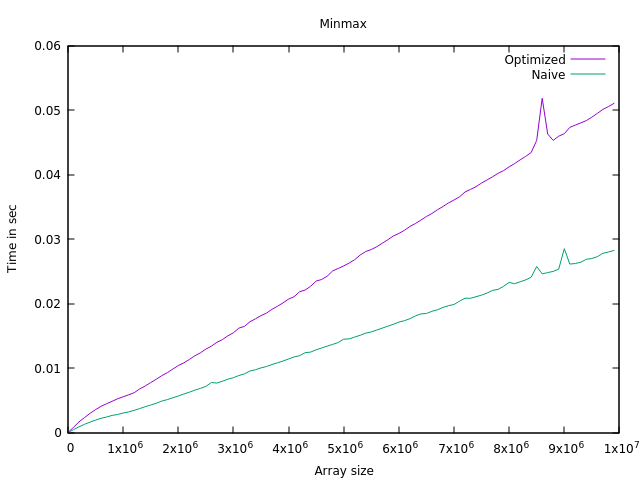
\includegraphics[width=0.75\textwidth]{minmax10m_c.png}
\end{figure}

\item On veut montrer que le nombre d'erreurs de prédictions fait par le Minmax naïf est asymptotiquement équivalent à $4\log n$, et que le nombre d'erreurs de prédictions fait par le Minmax $\frac{3}{2}$ est asymptotiquement équivalent à $\frac{n}{4}$.

\begin{itemize}
\item Version naïve :

\begin{itemize}[label=$\bullet$]
\item On établit une correspondance entre les éléments d'une permutation et les cycles d'un graphe. \\
Pour cela, on définit une bijection f qui part de l'ensemble des permutations de taille n vers lui-même tel
que le nombre de min-records dans $f(\sigma)$ soit égal au nombre de cycles de $\sigma$.
\item Pour $\zeta$ une variable aléatoire réelle à valeur dans l'ensemble de permutations uniformes aléatoires,
on considère son espérance $E_n[\zeta]$.

\item On veut compter le nombre d'erreurs de prédictions $\zeta(f(\sigma))$ provoqué par la ligne 3 de l'algorithme naïf cycle par cycle.
\item On compte au total 4 erreurs de prédictions suivant l'état de départ du prédicteur et la longueur des cycles étudiés.
\item Le nombre d'erreurs de prédictions de $f(\sigma)$ est égal à quatre fois le nombre de cycles de la permutation $\sigma$ $(Cyc)$.
\item L'espérance de Cyc $E_n[Cyc]$ étant équivalent à $\log n$, on en déduit que le Minmax naïf fait en moyenne $4\log n$ erreurs de prédiction.
\end{itemize}

\item Version optimisée : 

Le premier test en ligne 3 de l'algorithme $\frac{3}{2}-MINMAX$ provoque une erreur de prédiction avec une probabilité de
$\frac{1}{2}$, comme ce test est répété sur tout le tableau deux par deux éléments, $\frac{3}{2}-MINMAX$ provoque $\frac{1}{2} \frac{n}{2} = \frac{n}{4}$
erreurs de prédiction.
\end{itemize}


    \item Les expérimentations ont été reproduites en utilisant Python. \\
            L'algorithme optimisé est plus lent, mais l'écart avec la version naïve est moindre
            comparé à l'implémentation en C.

\begin{figure}[!ht]
  \caption{Performance des implémentations en Python des deux algorithmes}
\centering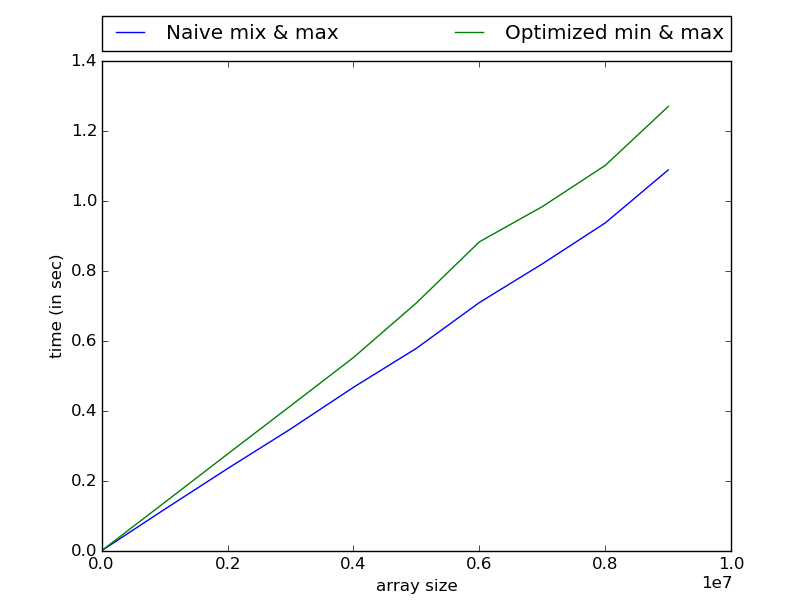
\includegraphics[width=0.75\textwidth]{minmax10m_py.png}
\end{figure}

	\item On devrait s'attendre à ce que l'algorithme naïf soit moins performant que l'algorithme optimisé en nombre de comparaisons. \\
    Mais l'implémentation de l'algorithme de comparaison des arbres unaire-binaires attendue n'est pas correcte.

\begin{figure}[!ht]
  \caption{Performance des implémentations des deux algorithmes en Python opérant sur des arbres unaires-binaires.}
\centering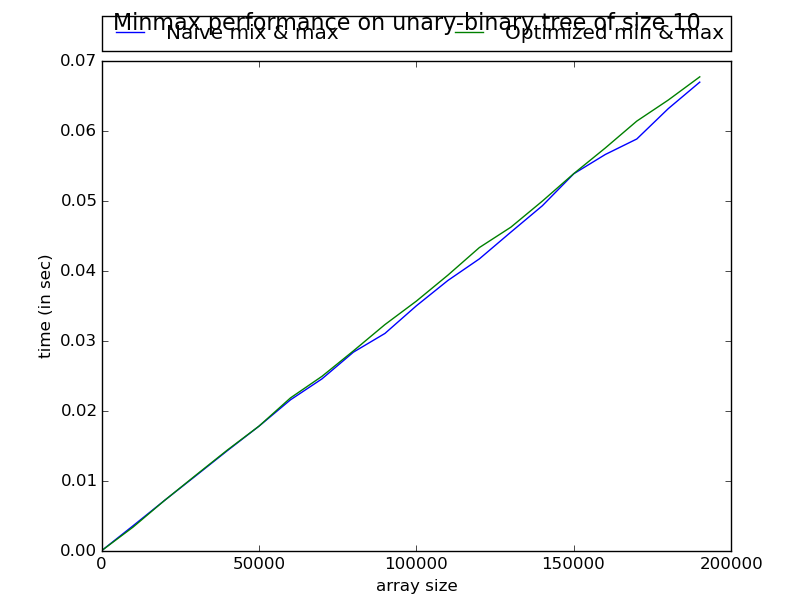
\includegraphics[width=0.75\textwidth]{aubminmax200k_py.png}
\end{figure}

	\item Voir 5.

\section{Exponentiation rapide}

	\item Pour la suite de la section, le problème de l'exponentiation rapide a été choisi.

   	\item

\begin{itemize}
    \item L'algorithme naïf : on multiplie un nombre x par lui-même un nombre n de fois dans une boucle.
    \item La version optimisée: Considérant une fonction récursive expsqu(x, n) qui prend un entier n supérieur à 1 et un réel
x en paramètres. On distingue 3 cas pour n:
\begin{itemize}[label=$\bullet$]
\item Si n = 1, on renvoie x. (expsqu(x, 1) = x)
\item Si n est pair, on calcule \( (x^2)^{n/2} \), soit expsqu( \(x^2\), n/2 ),
\item Si n est impair avec n > 2, on calcule \( x(x^2)^{(n-1)/2} \), soit x $\cdot$ expsqu( \( x^2 \), (n-1)/2 ).
\end{itemize}
\end{itemize}

	\item{
\begin{itemize}
    \item La version naïve a une complexité temporelle linéaire en \BigO{n} avec n - 1 multiplications.
    \item
 La version optimisée a une complexité temporelle en \BigO{\log _2 \left( n \right )}, avec
    au plus $\lfloor \log _2 \left( n \right ) \rfloor$ multiplications et $\lfloor \log _2 \left( n \right ) \rfloor$ élévations au carré.
\end{itemize}}

\clearpage

	\item Les résultats semblent correspondre à ceux des expérimentations réalisées par les auteurs de l'article.

\begin{figure}[h]
  \caption{Performance des algorithmes d'exponentiation rapide en C (50 millions de calculs)}
\centering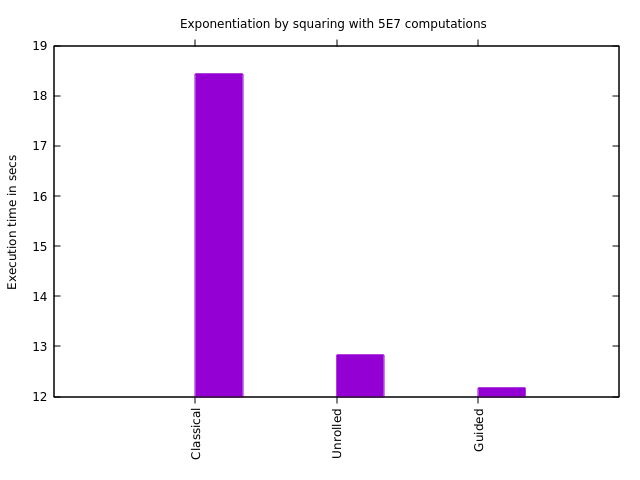
\includegraphics[width=0.75\textwidth]{expsqu50m_c.png}
\end{figure}

    \item Les implémentations Python sont plus lentes, mais en plus les vitesses d'éxecution des
 différentes implémentations ne diffèrent pas tant que cela. Ici, l'algorithme guidé est même plus
rapide que l'algorithme déroulé, alors que en C il s'agit de l'algorithme le plus rapide.
Serait-ce dû à l'utilisation d'un language interprêté? Les opérations logiques semblent plus rapides
que des divisions entières.

\lstset{language=bash}          
\begin{lstlisting}[frame=single]
% python3 -m timeit -n 100000000 -s 'x = 47' 'x // 2'
100000000 loops, best of 3: 0.0597 usec per loop
% python3 -m timeit -n 100000000 -s 'x = 47' 'x >> 1'
100000000 loops, best of 3: 0.0485 usec per loop
% python3 -m timeit -n 100000000 -s 'x = 47' 'x // 4' 
100000000 loops, best of 3: 0.0601 usec per loop
% python3 -m timeit -n 100000000 -s 'x = 47' 'x >> 2'
100000000 loops, best of 3: 0.048 usec per loop
\end{lstlisting}

\clearpage

\begin{figure}[h]
  \caption{Performance des algorithmes d'exponentiation rapide en Python (50 millions de calculs)}
\centering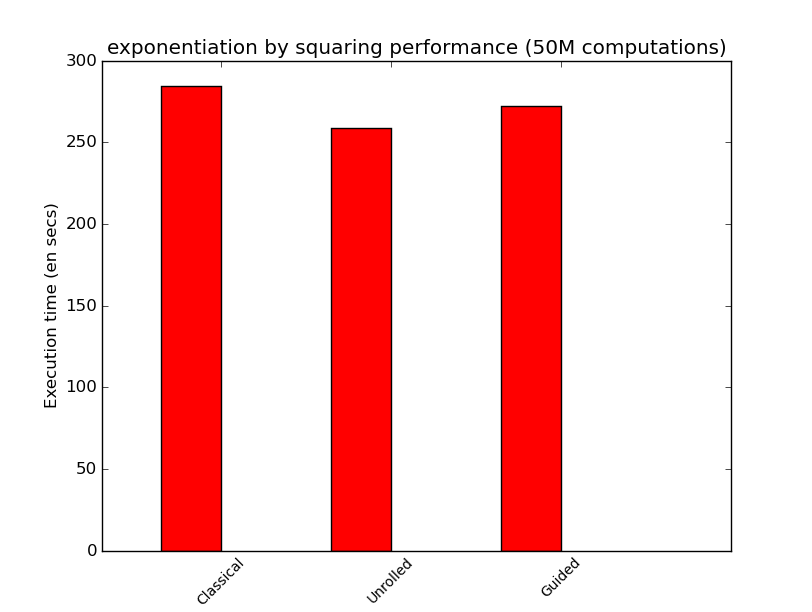
\includegraphics[width=0.75\textwidth]{expsqu50m_py.png}
\end{figure}

\section{Au-delà de l’article}
\subsection{Somme maximale}

	\item

\begin{itemize}
    \item La version naïve : on utilise deux boucles avec deux indices, l'indice de la première boucle
indique le premier élément du sous-tableau étudié, l'indice de la deuxième boucle basé sur le premier
indice indexe le sous-tableau défini dans la première boucle, calcule la somme des éléments du sous-tableau,
puis compare cette somme à une variable contenant la somme maximale courante. Cette somme est mise à jour
si la somme calculée est supérieure.
    \item La version optimisée : 
\begin{itemize}[label=$\bullet$]
\item On calcule l'indice qui représente l'élément du milieu du tableau.
\item On définit une fonction utilitaire appelée max\_crossing\_sum qui renvoie la somme maximale d'un tableau en y incluant l'élément
du milieu du tableau.
\item On divise le tableau en deux moitiés, puis on fait un appel récursif sur chaque moitié.
\item On renvoie le maximum de ces deux résultats et du résultat de max\_crossing\_sum.
\end{itemize}
\end{itemize}

   	\item
\begin{itemize}
\item La version naïve a une complexité temporelle quadratique en \BigO{n^2}.
\item La version optimisée : on a une complexité quasilinéaire en $\theta ( n \cdot \log _2 \left( n \right ) )$ obtenue
à partir de la relation de récurrence $ T(n) = 2 \cdot T(n/2) + \theta (n)$ et du cas 2 du théorème maître.
\end{itemize}

   	\item Les résultats sont surprenants : pourquoi est-ce la version optimisée s'éxecute en temps constant,
et pourtant donne les mêmes résultats que la version naïve en C comme en Python?
Cela ne correspond pas à ce qui a été prédit précédemment.
En tout cas, l'algorithme de somme maximale ne semble pas être handicapé par les erreurs de prédictions.

\begin{figure}[h]
  \caption{Performance des algorithmes de somme maximale en C}
\centering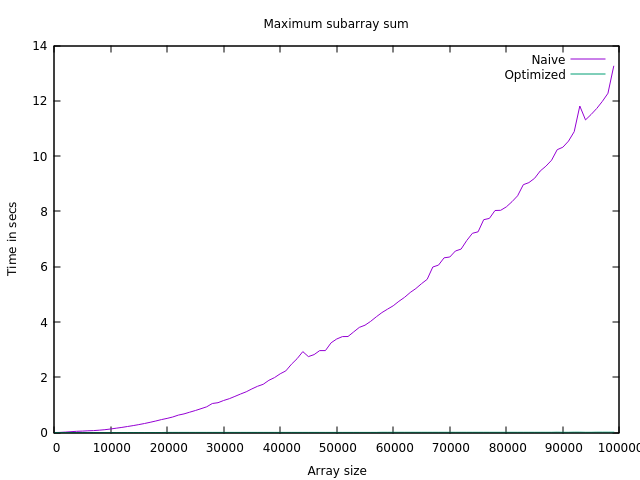
\includegraphics[width=1\textwidth]{subarray100k_c.png}
\end{figure}

\begin{figure}[h]
  \caption{Performance des algorithmes de somme maximale en Python}
\centering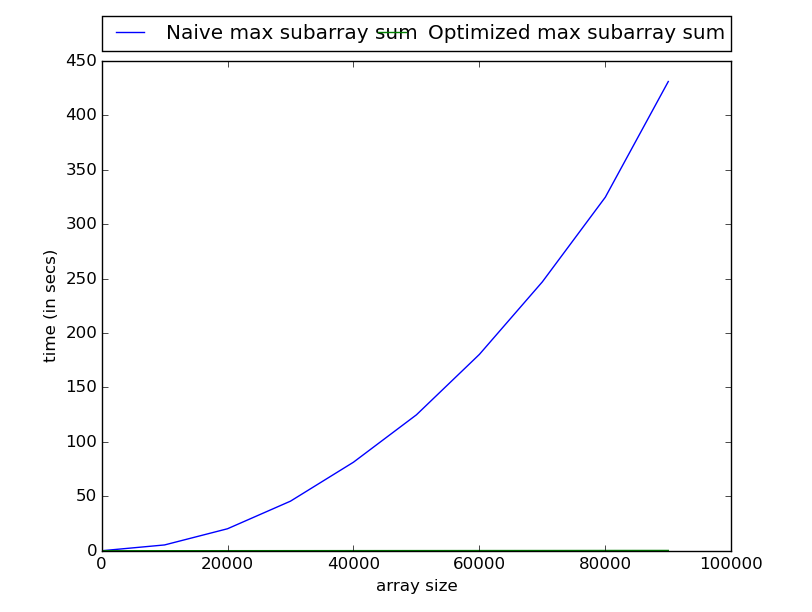
\includegraphics[width=1\textwidth]{subarray100k_py.png}
\end{figure}


\end{enumerate}

\end{document}
